\chapter{Implementation} 
\label{chapter:implementation}
This chapter describes the design of smart contracts and provides the detailed implementation of each function that is adopted in this paper. The smart contract diagram as shown in Figure~\ref{fig:smart_contract_diagram},  all of the organizations have common \(OMgr\) for managing users' information and storing users' status. The ecosystem initiator enables blockchain-based functionality by deploying a \(OMgr\). It offers application binary interface (ABI) files for all participants to easily call smart contract functions.

\begin{figure}[hb]
    \centering
    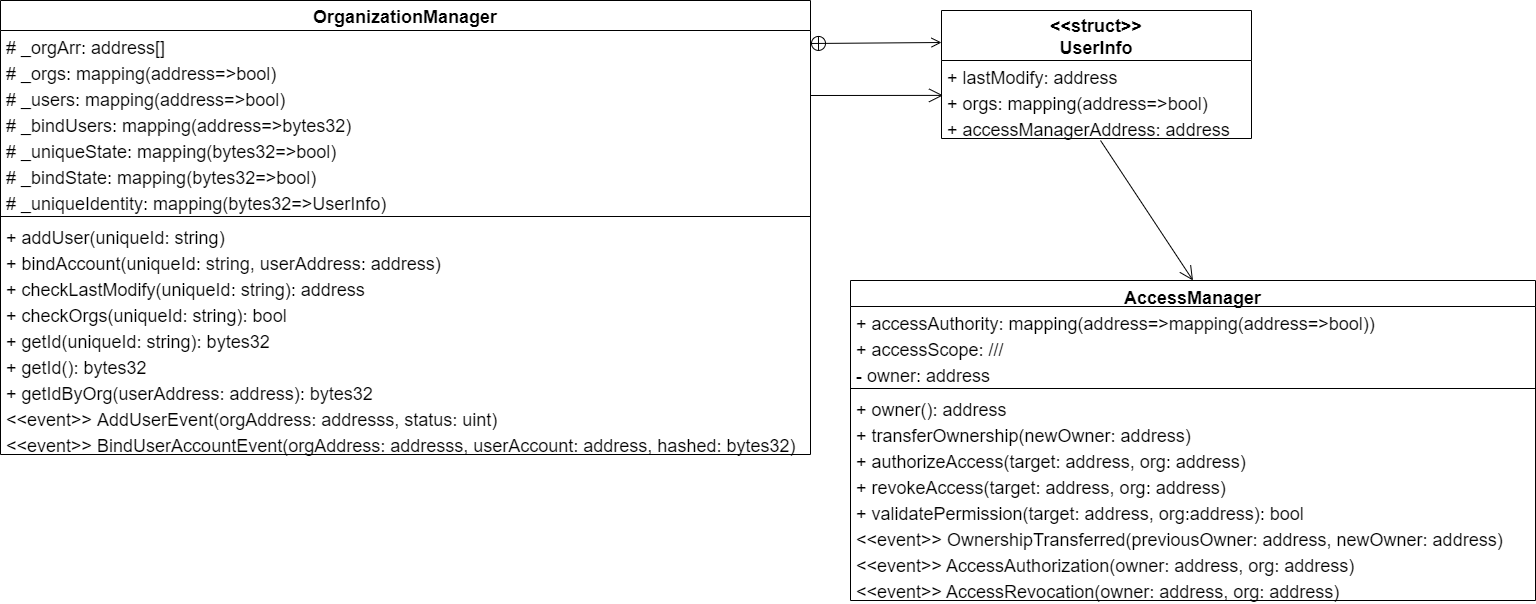
\includegraphics[height=!,width=1\linewidth,keepaspectratio=true]{figures/smart_contract_diagram.png}
    \caption{{\footnotesize Smart Contract Diagram}}
    \label{fig:smart_contract_diagram}
\end{figure}
\section{Smart contract design}
\subsection*{Organization Manager}
The \(OMgr\) is used to manage information that is related to users and organizations, i.e., it records data attributes, users' identity hash value. In Table~\ref{table:userinfo}, the \textit{UserInfo} structure represents an independent \(DI\). After the identity verification process is done as shown in Figure~\ref{fig:identityVerification}, the \(DI\) will be created for users automatically.\par
Because every organization has one key pair for determined their identity, we can retrieve their address from the private key and then append these addresses to the variable \(orgs\) in \(OMgr\).\par

\begin{table}[h]
     \centering
     % [] 顯示在 list of tables 的文字
     % {} 顯示在表格上方的文字
     \caption[Table of UserInfo structure]{Table of \textit{UserInfo} structure}
     \label{table:userinfo}
     \begin{tabular}{lll}
     \toprule[1.1pt]
                   Variable & Type & Description\\
     \midrule[1.1pt]
     \textit{lastModify}     & address   & \begin{tabular}[c]{@{}l@{}} Address of last organization that\\ verifies the user\end{tabular}\\                                
     \midrule
     \multirow{1}{*}{\textit{orgs}} & mapping(address==>bool) & Organization's mapping\\
     \midrule
     \multirow{1}{*}{\textit{userAddress}} & address & Corresponding Ethereum address\\
     \midrule
     \multirow{1}{*}{\textit{accessManagerAddress}} & address & Address of $ACMgr_i$ contract\\          
     \bottomrule[1.1pt]
     \end{tabular}
     \end{table}

This smart contract provides functions to create user identity, bind account with Ethereum address, and create exclusive \(ACMgr\) for the user as shown in Figure~\ref{fig:smart_contract_deployment}. And it also defines events in order that the smart contract can emit events to record logs on the block. That enables traceability of identity creation processes. The most important functions we used in \(OMgr\) are \textit{addUser}, \textit{bindAccount} and only the legitimate organizations are able to trigger these functions.\par 
The function \textit{addUser} is invoked after finishing identity verification, the \(OMgr\) check whether the \(ID\) exist on the blockchain. Then if the \(ID\) is new one, the \(OMgr\) will create \textit{UserInfo} for users. Otherwise, the \(OMgr\) will append the address of \(Org\) who triggers this function to the variable \textit{orgs} in \textit{UserInfo}.\par 
The function \textit{bindAccount} is used to bind user's \(DI\) to Ethereum address. So that every contract \(ACMgr\) will record organizations which the user has registered. One \(DI\) only corresponds to one Ethereum address,  to establish a contract for storing access right.\par 

\subsection*{Access Manager}
After binding to address, contract \(ACMgr\) will be created and required to transfer ownership of this contract, i.e., the user has full right to manage its contract and authorize access right to any legitimate organization. And users have a full right to make their choice as to whether or not to allow personal data opened. This contract uses two mappings to store access right in the form of key and value pairs where every key is unique. These keys represent attribute names that \(RA\) approves and submits. It is necessary to formulate data attributes for users and organizations by \(RA\) because financial data attributes will update dynamically and only \(RA\) can update these attributes. For example, the Financial Supervisory Commission (FSC) was in charge of the development, supervision, regulation, and examination of financial services in Taiwan.

\begin{figure}[htb]
    \centering
    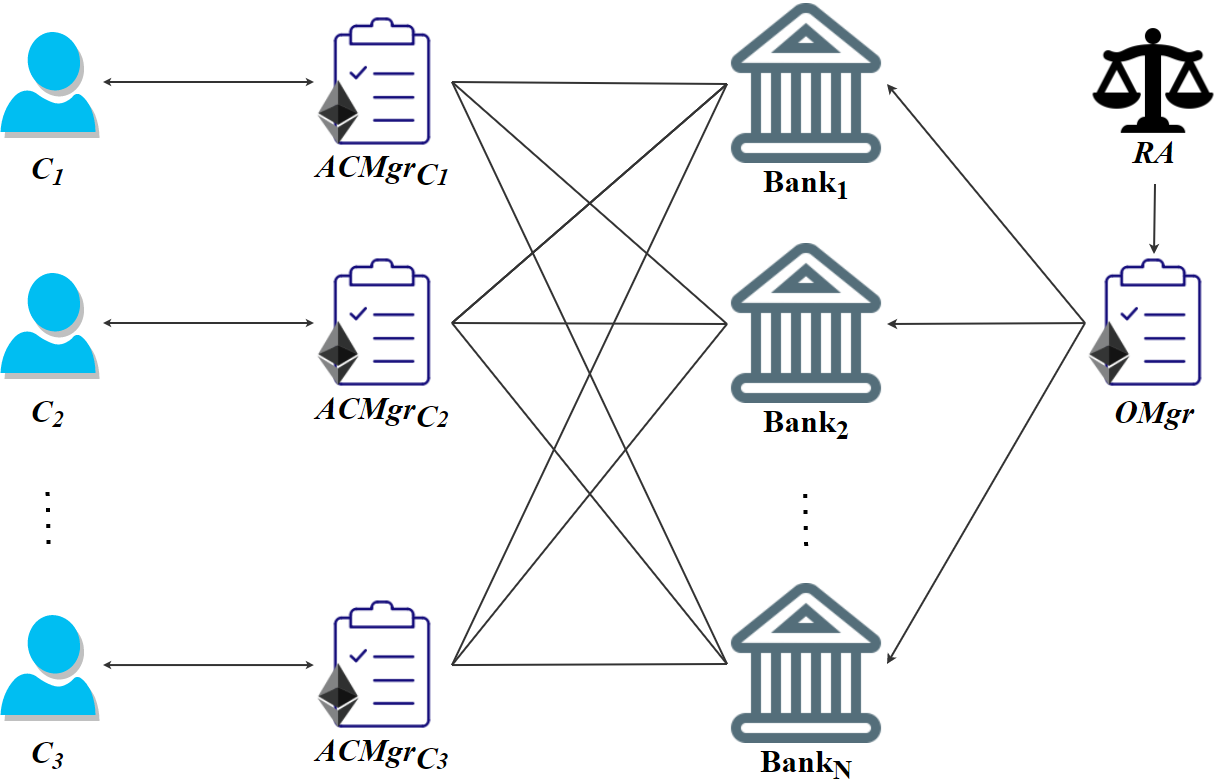
\includegraphics[height=!,width=0.8\linewidth,keepaspectratio=true]{figures/smart_contract_deployment.png}
    \caption{{\footnotesize The relation between smart contracts}}
    \label{fig:smart_contract_deployment}
\end{figure}
For the purpose of delivering a better user experience, we designed two access authorization modes for access personal data. If the \(C_N\) want to allow \(TSP\) to access the data from all \(Org\) ($Bank$), the \(C_N\) needs to authorize access many times due to one on one authorization, it is called Mode 1 as shown in Table~\ref{table:accessStruct}. Another mode is one-to-many, the user only needs to select the attribute name that the user wants to share. Afterward, all the legitimate banks will accept any data request from \(TSP\)  against the selected attribute.
\begin{table}[h]
    \centering
    % [] 顯示在 list of tables 的文字
    % {} 顯示在表格上方的文字
    \caption[Table of access right structure]{Table of access right structure}
    \label{table:accessStruct}
    \begin{tabular}{llll}
    \toprule[1.1pt]
                  Variable & Type & Mode\\
    \midrule[1.1pt]
    \multirow{1}{*}{\textit{accessAuthority}} & mapping(string=>mapping(address=>mapping(address=>bool))) & Mode 1\\ 
    \midrule
    \multirow{1}{*}{\textit{oneApproved}} & mapping(string=>bool) & Mode 2\\
    \bottomrule[1.1pt]
    \end{tabular}
    \end{table}

\newpage

\section{Third Party Login}

\begin{figure}[htb]
    \centering
    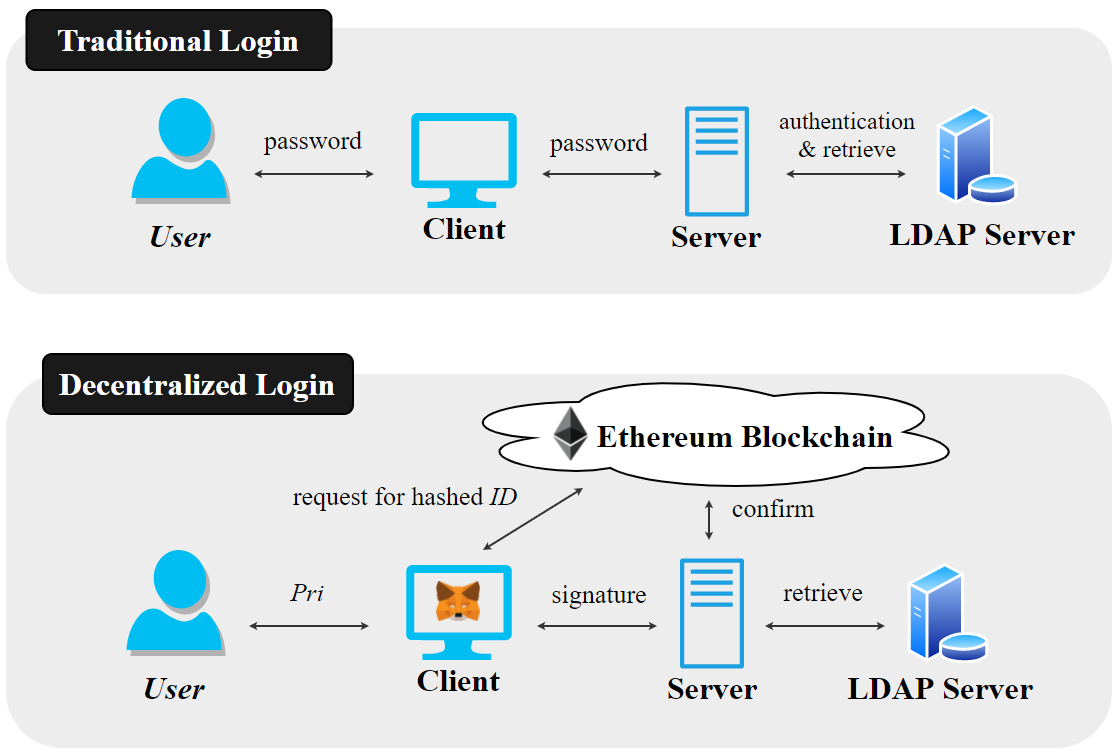
\includegraphics[height=!,width=1\linewidth,keepaspectratio=true]{figures/traditional_decentralized.png}
    \caption{{\footnotesize Traditional vs. Decentralized login}}
    \label{fig:traditional_decentralized}
\end{figure}

In contrast to traditional login as shown in Figure~\ref{fig:traditional_decentralized}, the user can log in to other organizations with decentralized login and it doesn't need to remember any password, because the unique \(DI\) store on blockchain and the server can verify the user's identity by validating the signature that the user sign its hashed \(ID\).\par
Our framework supports both of login mechanisms and utilizes hashed \(ID\) as the primary key to restoring user account information that the user stores on the LDAP server. Before binding account, the hashed \(ID\) doesn't establish yet and leave the hashed field empty.\par 
To begin this decentralized login process, the client should install the MetaMask extension on Chrome browser and import existed private key or register a new one. The first step in this process was to use \textit{call} function to view the user's hashed \(ID\) from blockchain. The second step was to sign the hashed \(ID\) by the user's private key using ECDSA. The final step was confirm with blockchain by server and then retrieve user account information.

\section{Account Integration}
In existing systems, users have an obligation to remember their own username/password pairs as users register a new one. Furthermore, because these pairs are following different rules, such as at least upper and lower case letters, character, symbol. It would be difficult for users to manage these pairs that are distributed and messy. There are several tangible solutions for storing these pairs nowadays. For instance, 1password and LastPass are password managers that save your username and password to cloud storage. But they cost money and users are required to trust a third party that controls their personal information. Besides, some services and platforms have already had their extreme vulnerability. Instead, we propose an account integration solution, which makes use of blockchain technology to generate tamper-proof record and realize access control.\par 
In order to effectively perform account integration without a single authority entity, we took advantage of a secure hash algorithm and blockchain smart contracts that execute when the specific conditions are met. In the proposed architecture, the user has a secure and convenient way to build their own account integration via smart contracts on the blockchain, as depicted below.

\renewcommand\labelenumi{(\theenumi)}
\begin{enumerate}[noitemsep, topsep=0pt]
    \item A \(C_i\) registers organization accounts respectively, these accounts are relatively independent of each other.
    \item One of the organizations creates DI using a hash algorithm Keccak-256  on blockchain as \(C_i\) passes real-name authentication, the others append their organization address to the same DI.
    \item After establishing an identity, the \(C_i\) will propose an account binding request when the \(C_i\) wants to participant in this ecosystem.
    \item One organization that the \(C_i\) registers with receives this request and then creates a transaction signed by its organization's private key to bind these accounts to the Ethereum address that the \(C_i\) specify. 
    \item Afterward, the \(C_i\) can use the bound address to sign in or sign up for organizations within this ecosystem.
\end{enumerate}

\begin{figure}[htb]
    \centering
    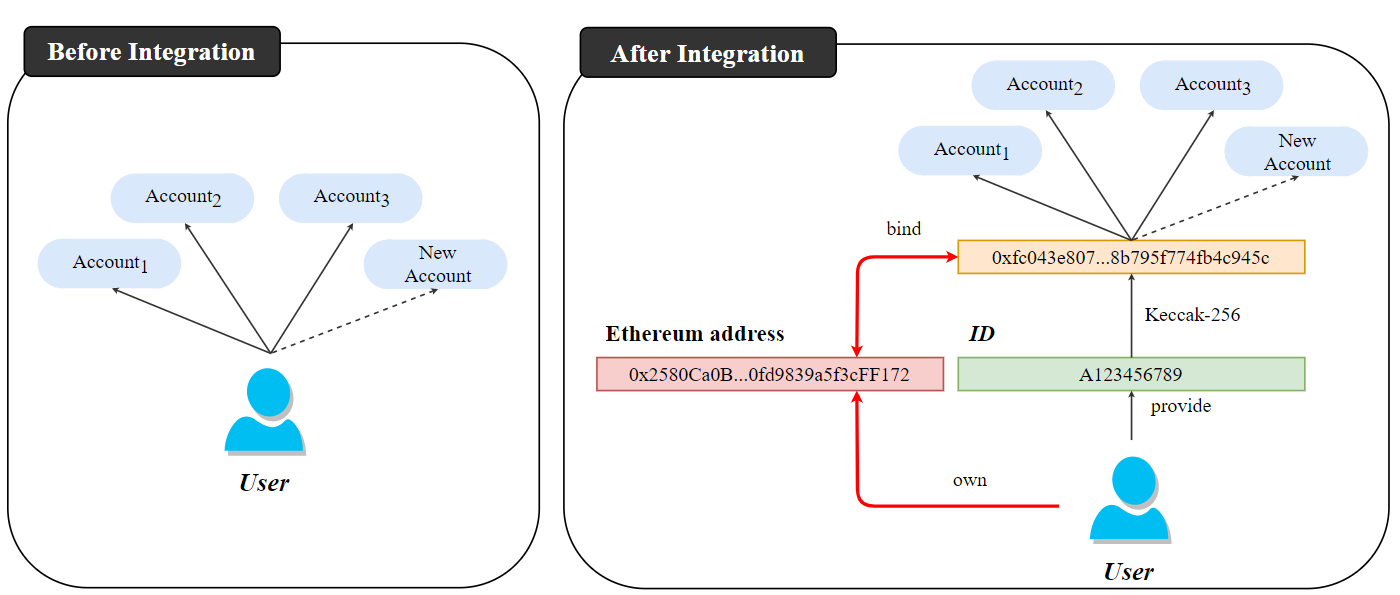
\includegraphics[height=!,width=1\linewidth,keepaspectratio=true]{figures/account_integration.png}
    \caption{{\footnotesize Account integration}}
    \label{fig:account_integration}
\end{figure}

As the Figure~\ref{fig:account_integration} shows a scenario, where a user uses the bound address to find an organization account for sign-in organization's service.  This account integration has brought benefits to users such as ease of management, sign-up without additional registration, as well as no more information to be revealed to the public.

\newpage
\section{Data Sharing}
Since our proposed system needs a secure transmitting mechanism for transmitting users' personal information such as financial data and better performance to reduce network latency that transmission need, the JSON Web Token (JWT) was adopted to verify the owner of JSON data. In our proposed system, the authentication module will allow TSPs to perform challenge response authentication in order to obtain a JWT which allows TSPs to access a specific resource from the organization without authenticating again. Once JWT has been obtained from the organization, the TSP can send a request using the JWT to fetch data for a period of time.\par  
Conventionally, a solution was used to do authentication between client and server, called a session. It is used by the server to maintain the status of the client and the session is stored on the server. Although it may cause performance overhead in the case of large volumes of users by storing much session data on the server's memory, it still works for most applications. Our application has made use of sessions once the user has authenticated, i.e., the user login service.\par
Although session technology solves authentication issues well, we have different requirements for our data sharing schema. In our scenarios, one application is required to communicate with multiple authentication servers to get corresponding tokens as shown Figure~\ref{fig:jwt_flow}. Specifically, in a single user's data request, the TSP's server should send access token requests many times and keep them in the database for later use (see sample in Figure~\ref{fig:screenshot_database}). \par
\begin{figure}[htb]
    \centering
    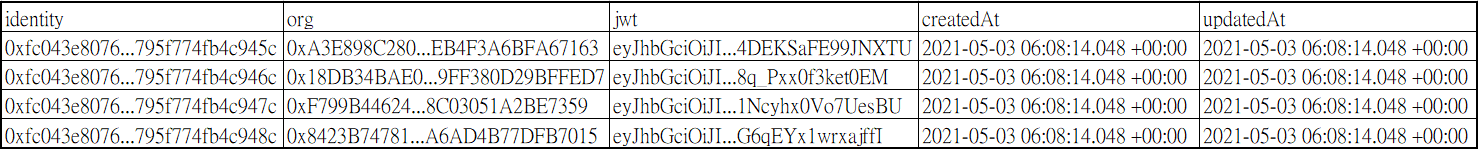
\includegraphics[height=!,width=1\linewidth,keepaspectratio=true]{figures/screenshot_database.png}
    \caption{{\footnotesize Screenshot of token database in TSP}}
    \label{fig:screenshot_database}
\end{figure}

Therefore, instead of using the session for authentication of data sharing, we take advantage of JWT to issue access tokens. The JWT is a self-contained token that has authentication information, expiration time, and other user-defined claims digitally signed. As illustrated in Table~\ref{table:jwt}, each JWT contains these claims for specifying the entity which the TSP wants to query. The \textit{hashed} value is used to identify the data owner thereby the TSP can access the user's data without more detailed information about the user.\par
\begin{table}[h]
    \centering
    % [] 顯示在 list of tables 的文字
    % {} 顯示在表格上方的文字
    \caption[JWT claims used in our system]{JWT claims used in our system}
    \label{table:jwt}
    \begin{tabular}{lll}
    \toprule[1.1pt]
                  Name & Type & Semantics\\
    \midrule[1.1pt]
    \textit{hashed}     & byte32   &  The hash value of user's \(ID\). For example,\\
    & & 0xfc043e80768cb3034a508ca5e0e256c5c72aad2642771f18b795f774fb4c945c \\
    \midrule
    \multirow{1}{*}{\textit{iat}} & timestamp & The time at which the JWT was issued.\\
    \midrule
    \multirow{1}{*}{\textit{exp}} & timestamp  & The expiration time of the JWT\\
    \midrule
    \multirow{1}{*}{\textit{iss}} & address & The issuer of the JWT. For example,\\
    & & 0x1F7F0F7BE634D340EB070F3F3C21B6CE4AB857BD\\      
    \midrule
    \multirow{1}{*}{\textit{sub}} & address & The subject of the JWT, i.e., the TSP that will use the JWT. For example,\\
    & & 0xA3E898C280220BF5FAE9E7E6CEB4F3A6BFA67163\\
    \bottomrule[1.1pt]
    \end{tabular}
    \end{table}

After the user agrees to grant access permission for the TSP via \textit{ACMgr} contract, the user will inform the TSP to send requests to all organizations via the states of the user's \textit{ACMgr} contract and configuration file. The mapping of address of the organization and IP address as shown in Figure~\ref{fig:mappingExample} to specify the corresponding IP address of the organization. Currently, these configuration files are stored on each organization's servers. \par
When the TSP is required to access the user's data, it just reuses this token to fetch data if the JWT doesn't expire. The issuer of the JWT will give a specific expiration instant. In most applications, it is recommended to set it smaller (a few minutes). It will need to balance tradeoffs with performance and security. Although JWT brings us a lot of benefits such as superior performance, portable, decentralized, the drawback of JWT is token revocation. This implies that a JWT that organization issued can be valid even if the user takes back the access permission. In order to overcome this drawback, we enable blockchain technology to verify the token. In addition to verifying tokens by the authentication server, our system also verifies tokens with \textit{ACMgr} contract via a function call. The overhead of a function call of the smart contract will be compared in a later chapter.\par
\begin{figure}[htb]
    \centering
    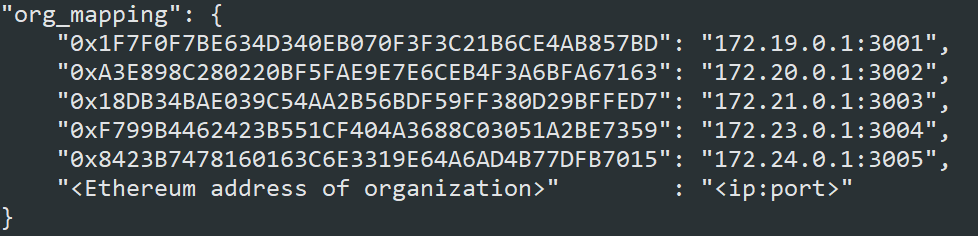
\includegraphics[height=!,width=0.9\linewidth,keepaspectratio=true]{figures/mapping_example.png}
    \caption{{\footnotesize Example of organization mappiing}}
    \label{fig:mappingExample}
\end{figure}
\newpage
\begin{figure}[htb]
    \centering
    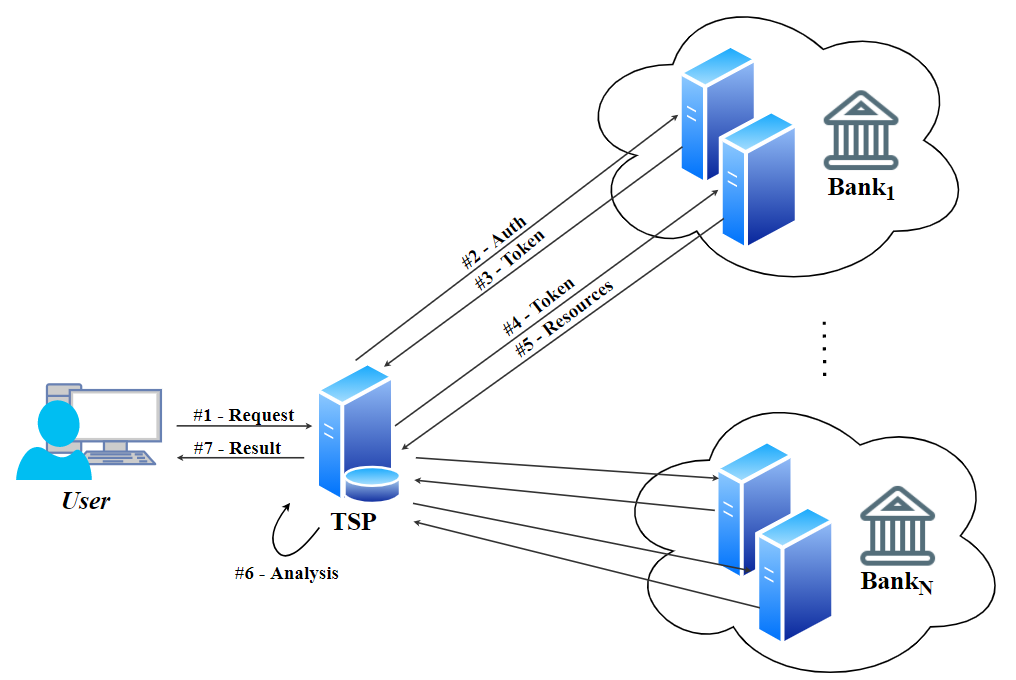
\includegraphics[height=!,width=1\linewidth,keepaspectratio=true]{figures/jwt_flow.png}
    \caption{{\footnotesize A user send a request for data}}
    \label{fig:jwt_flow}
\end{figure}
The Figure~\ref{fig:jwt_flow} shows that a user sends a request to the TSP server, which will initiate subsequent requests to retrieve JWTs. Firstly, the server has to perform authentication until it collects all JWTs. If one of the requests is failed, just ignore the request failure and report it to the user. It won't affect other normal requests. Secondly, the JWTs can be utilized in two modes. In other words, we do not have to create two kinds of JWT for different modes. Because the JWT doesn't contain access right scope or other credential information. To perform secure data sharing, we have chosen the API to share data between parties. For more flexibility in this framework, we support three ways to let TSPs attach a JWT to the calling API: (1) as a query string parameter. (2) a form body parameter. (3) \textit{x-access-token} header. Table~\ref{table:api} shows the APIs used in our framework, the query string parameter \textit{ACMgr} stands for the specific user's contract address.
\begin{table}[h]
    \centering
    % [] 顯示在 list of tables 的文字
    % {} 顯示在表格上方的文字
    \caption[APIs used in data sharing]{APIs used in data sharing}
    \label{table:api}
    \begin{tabular}{llll}
    \toprule[1.1pt]
                  Name & Method & Description & Mode\\
    \midrule[1.1pt]
    \multirow{1}{*}{/users/protected?acc=\{\textit{ACMgr}\}} & GET & Get the user's deposit value & Mode 1\\
    \midrule
    \multirow{1}{*}{/users/protectedInvoice?acc=\{\textit{ACMgr}\}} & GET & Get the user's bill & Mode 2\\
    \bottomrule[1.1pt]
    \end{tabular}
    \end{table}